%%%%%%%%%%%%%%%%%%%%%%%%%%%%%%%%%%%%%%%%%
% Modelo de Trabalho de Conclusão de Curso
% Bacharelado em Sistemas de Informação - IFNMG - Campus Salinas
% Classe abnTeX2 (ABNT NBR 14724:2011, NBR 6028:2021, NBR 10520:2023)
%
% Modelo adaptado de:
% Frits Wenneker (http://www.howtotex.com)
%
% License:
% CC BY-NC-SA 3.0 (http://creativecommons.org/licenses/by-nc-sa/3.0/)
%
% Compilação: pdflatex -> bibtex -> pdflatex -> pdflatex (ou latexmk -pdf main.tex)
%%%%%%%%%%%%%%%%%%%%%%%%%%%%%%%%%%%%%%%%%


\documentclass[
	% -- opções da classe memoir --
	12pt,				% tamanho da fonte
	%openright,			% capítulos começam em pág ímpar (insere página vazia caso preciso)
	twoside,			% para impressão em recto e verso. Oposto a oneside
	a4paper,			% tamanho do papel.
	% -- opções da classe abntex2 --
	chapter=TITLE,		% títulos de capítulos convertidos em letras maiúsculas
	section=TITLE,		% títulos de seções convertidos em letras maiúsculas
	subsection=TITLE,	% títulos de subseções convertidos em letras maiúsculas
	subsubsection=TITLE,% títulos de subsubseções convertidos em letras maiúsculas
	% -- opções do pacote babel --
	english,			% idioma adicional para hifenização
	french,				% idioma adicional para hifenização
	spanish,			% idioma adicional para hifenização
	brazil,				% idioma principal (o nome "brazil" é exigido pela classe abntex2,
						% que define \captionsbrazil internamente)
	]{abntex2}

% ---------------------------------
% Quadros (ilustração textual, NBR 14724)
% Definido antes do pacote float, que redefine \newfloat do memoir
% ---------------------------------
\newcommand{\quadroname}{Quadro}
\newcommand{\listofquadrosname}{Lista de quadros}
\newfloat[chapter]{quadro}{loq}{\quadroname}
\newlistof{listofquadros}{loq}{\listofquadrosname}
\newlistentry{quadro}{loq}{0}
\counterwithout{quadro}{chapter}
\renewcommand{\cftquadroname}{\quadroname\space}
\renewcommand*{\cftquadroaftersnum}{\hfill\textendash\hfill}

% ---------------------------------
% PACOTES
% ---------------------------------
\usepackage{lmodern}			% Usa a fonte Latin Modern
\usepackage[T1]{fontenc}		% Seleção de códigos de fonte
\usepackage{indentfirst}		% Indenta o primeiro parágrafo de cada seção
\usepackage[table]{xcolor}		% Controle das cores (inclui cores em tabelas)
\usepackage{lastpage}
\usepackage{graphicx}			% Inclusão de gráficos
\usepackage{microtype} 			% Melhorias de justificação
\usepackage{amsmath,amsfonts,amssymb}
\usepackage{multirow}           % Mesclar linhas e colunas em tabelas
\usepackage{longtable}          % Tabelas longas
\usepackage{fancyvrb}           % Saídas e comandos
\usepackage{pdflscape}          % Páginas em paisagem
\usepackage{float}
\usepackage{subcaption}         % Subfiguras
\usepackage{booktabs}           % Linhas de tabelas
\usepackage[portuguese, ruled, linesnumbered]{algorithm2e}
\usepackage{csquotes}           % Aspas corretas (\enquote)

% ---------------------------------
% Pacotes de citações
% ---------------------------------
\usepackage[brazilian,hyperpageref]{backref}% Páginas com as citações na bibliografia
\usepackage[alf,bibjustif]{abntex2cite}	% Citações padrão ABNT

% ---------------------------------
% Configurações do pacote backref
% ---------------------------------
\renewcommand{\backrefpagesname}{Citado na(s) página(s):~}
\renewcommand{\backref}{}
\renewcommand*{\backrefalt}[4]{
	\ifcase #1 %
		Nenhuma citação no texto.%
	\or
		Citado na página #2.%
	\else
		Citado #1 vezes nas páginas #2.%
	\fi}%

%-----------------------------------
% Dados do trabalho
%-----------------------------------
\titulo{Título do Trabalho}
\autor{Nome do Autor}
\local{Salinas - Minas Gerais}
\data{\the\year}                % ABNT: apenas o ano de depósito
\orientador{Prof. Dr. Nome do Orientador}
%\coorientador{Prof. Dr. Nome do Coorientador} % descomente se houver coorientador
\instituicao{%
	Instituto Federal do Norte de Minas Gerais - Campus Salinas
	\par
	Bacharelado em Sistemas de Informação
}
\tipotrabalho{Trabalho de Conclusão de Curso}
\preambulo{Trabalho de conclusão de curso apresentado ao Curso de Bacharelado em Sistemas de Informação do Instituto Federal do Norte de Minas Gerais, como exigência para obtenção do grau de Bacharel em Sistemas de Informação.}

%-----------------------------------
% Aparência do PDF final
%-----------------------------------
\definecolor{blue}{RGB}{41,5,195}

\makeatletter
\hypersetup{
	pdftitle={\@title},
	pdfauthor={\@author},
	pdfsubject={\imprimirpreambulo},
	pdfcreator={LaTeX with abnTeX2},
	pdfkeywords={abnt, latex, abntex, abntex2, trabalho acadêmico},
	colorlinks=true,        % false: links em caixas; true: links coloridos
	linkcolor=blue,         % links internos
	citecolor=blue,         % links para a bibliografia
	filecolor=magenta,      % links para arquivos
	urlcolor=blue,
	bookmarksdepth=4
}
\makeatother

%-----------------------------------
% Espaçamentos entre linhas e parágrafos
%-----------------------------------
\setlength{\parindent}{1.25cm}  % recuo de primeira linha
\setlength{\parskip}{0.2cm}     % espaço entre parágrafos

%-----------------------------------
% Documento
%-----------------------------------
\begin{document}

\selectlanguage{brazil}
\frenchspacing

%-----------------------------------
% ELEMENTOS PRÉ-TEXTUAIS (ordem da NBR 14724)
%-----------------------------------
\pretextual

% Capa
\imprimircapa

% Folha de rosto (o * indica que haverá a ficha catalográfica no verso)
\imprimirfolhaderosto*

%-----------------------------------
% Ficha catalográfica (verso da folha de rosto)
% Substitua pelo PDF fornecido pela biblioteca, por exemplo:
% \begin{fichacatalografica}
%     \includepdf{fichacatalografica.pdf}
% \end{fichacatalografica}
\begin{fichacatalografica}
	\sffamily
	\vspace*{\fill}
	\begin{center}
	\fbox{\begin{minipage}[c][8cm]{13.5cm}
		\small
		\imprimirautor
		\hspace{0.5cm} \imprimirtitulo  / \imprimirautor. --
		\imprimirlocal, \imprimirdata-

		\hspace{0.5cm} \pageref{LastPage} p. : il.

		\hspace{0.5cm} \imprimirorientadorRotulo~\imprimirorientador

		\hspace{0.5cm}
		\parbox[t]{12.5cm}{\imprimirtipotrabalho~--~\imprimirinstituicao,
		\imprimirdata.}

		\hspace{0.5cm}
			1. Palavra-chave1.
			2. Palavra-chave2.
			I. \imprimirorientador.
			II. \imprimirinstituicao.
			III. Título
	\end{minipage}}
	\end{center}
\end{fichacatalografica}

%-----------------------------------
% Folha de aprovação (obrigatória)
% Após a defesa, substitua pela versão assinada:
% \begin{folhadeaprovacao}
%     \includepdf{folhadeaprovacao_final.pdf}
% \end{folhadeaprovacao}
\begin{folhadeaprovacao}
	\begin{center}
		{\ABNTEXchapterfont\large\imprimirautor}

		\vspace*{\fill}\vspace*{\fill}
		\begin{center}
			\ABNTEXchapterfont\bfseries\Large\imprimirtitulo
		\end{center}
		\vspace*{\fill}

		\hspace{.45\textwidth}
		\begin{minipage}{.5\textwidth}
			\imprimirpreambulo
		\end{minipage}%
		\vspace*{\fill}
	\end{center}

	Trabalho aprovado. \imprimirlocal, \_\_ de \_\_\_\_\_\_\_\_ de \imprimirdata:

	\assinatura{\textbf{\imprimirorientador} \\ Orientador}
	\assinatura{\textbf{Professor} \\ Convidado 1}
	\assinatura{\textbf{Professor} \\ Convidado 2}

	\begin{center}
		\vspace*{0.5cm}
		{\large\imprimirlocal}
		\par
		{\large\imprimirdata}
		\vspace*{1cm}
	\end{center}
\end{folhadeaprovacao}

%-----------------------------------
% Dedicatória (opcional)
\begin{dedicatoria}
	\vspace*{\fill}
	\centering
	\noindent
	\textit{Dedicatória aqui...}
	\vspace*{\fill}
\end{dedicatoria}

%-----------------------------------
% Agradecimentos (opcional)
\begin{agradecimentos}
Agradecimentos...
\end{agradecimentos}

%-----------------------------------
% Epígrafe (opcional)
\begin{epigrafe}
	\vspace*{\fill}
	\begin{flushright}
		\textit{Epígrafe...}
	\end{flushright}
\end{epigrafe}

%-----------------------------------
% Resumo (NBR 6028:2021: parágrafo único, 150 a 500 palavras;
% palavras-chave separadas por ponto e vírgula e finalizadas por ponto)
\setlength{\absparsep}{18pt}

\begin{resumo}
	O resumo deve ser escrito em português, em parágrafo único, com 150 a 500 palavras, e apresentar de forma concisa o tema, os objetivos, os métodos empregados, os resultados e as conclusões do trabalho, permitindo ao leitor vislumbrar todo o conteúdo do documento. Deve ser uma versão precisa, sintetizada e seletiva do texto, dando destaque aos elementos mais importantes, redigida na voz ativa e na terceira pessoa do singular. Substitua este texto pelo resumo do seu trabalho.

	\textbf{Palavras-chave}: palavra-chave 1; palavra-chave 2; palavra-chave 3; palavra-chave 4; palavra-chave 5.
\end{resumo}

%-----------------------------------
% Abstract (resumo em língua estrangeira)
\begin{resumo}[Abstract]
	\begin{otherlanguage*}{english}
		An abstract is a self-contained, short, and powerful statement that describes a larger work. It should present the subject, objectives, methods, results, and conclusions of the work in a single paragraph. Replace this text with the English version of your abstract.

		\textbf{Keywords}: keyword 1; keyword 2; keyword 3; keyword 4; keyword 5.
	\end{otherlanguage*}
\end{resumo}

%-----------------------------------
% Lista de figuras
\pdfbookmark[0]{\listfigurename}{lof}
\listoffigures*
\cleardoublepage

%-----------------------------------
% Lista de quadros
\pdfbookmark[0]{\listofquadrosname}{loq}
\listofquadros*
\cleardoublepage

%-----------------------------------
% Lista de tabelas
\pdfbookmark[0]{\listtablename}{lot}
\listoftables*
\cleardoublepage

%-----------------------------------
% Lista de abreviaturas e siglas (opcional)
%-----------------------------------
% Lista de abreviaturas e siglas (ordem alfabética)
% Mantenha apenas as siglas efetivamente usadas no texto.
%-----------------------------------

\begin{siglas}
  \item[ABNT] Associação Brasileira de Normas Técnicas
  \item[BPMN] \textit{Business Process Model and Notation}
  \item[BSI] Bacharelado em Sistemas de Informação
  \item[CEP] Comitê de Ética em Pesquisa
  \item[IFNMG] Instituto Federal do Norte de Minas Gerais
  \item[LGPD] Lei Geral de Proteção de Dados Pessoais
  \item[PRISMA] \textit{Preferred Reporting Items for Systematic Reviews and Meta-Analyses}
  \item[SUS] \textit{System Usability Scale}
  \item[TCC] Trabalho de Conclusão de Curso
  \item[TCLE] Termo de Consentimento Livre e Esclarecido
\end{siglas}

\cleardoublepage

%-----------------------------------
% Lista de símbolos (opcional)
%-----------------------------------
% Lista de símbolos
% Mantenha apenas os símbolos efetivamente usados no texto.
%-----------------------------------

\begin{simbolos}
  \item[$ E $] Energia
  \item[$ m $] Massa
  \item[$ c $] Velocidade da luz no vácuo
\end{simbolos}

\cleardoublepage

%-----------------------------------
% Sumário
\pdfbookmark[0]{\contentsname}{toc}
\tableofcontents*
\cleardoublepage

%-----------------------------------
% ELEMENTOS TEXTUAIS
%-----------------------------------
\textual

\chapter{Introdução}
\label{cap1_introducao}

O objetivo deste documento é apresentar um modelo básico para a elaboração de Trabalho de Conclusão de Curso (TCC) do Instituto Federal do Norte de Minas Gerais (IFNMG), utilizando \LaTeX{} e a classe \textbf{abnTeX2}, em conformidade com as normas da Associação Brasileira de Normas Técnicas (ABNT), em especial a \texttt{ABNT NBR 14724:2011} (trabalhos acadêmicos) e a \texttt{ABNT NBR 10520:2023} (citações).

A introdução visa oferecer uma visão clara do que será tratado no trabalho e normalmente contempla os seguintes elementos:

\begin{alineas}
	\item \textbf{Contextualização do tema}: apresente o cenário atual do tema abordado, explicando sua relevância e o contexto no qual ele está inserido;
	\item \textbf{Problema de pesquisa}: defina de forma clara qual é o problema que o trabalho pretende abordar ou resolver, seja uma questão ou uma necessidade identificada na área de estudo;
	\item \textbf{Objetivo geral}: descreva o que o trabalho pretende alcançar de forma ampla;
	\item \textbf{Objetivos específicos}: detalhe as etapas ou os aspectos que devem ser abordados para atingir o objetivo geral;
	\item \textbf{Justificativa}: explique a relevância do trabalho, as possíveis contribuições para a academia, o mercado ou a sociedade e sua relação com outros estudos;
	\item \textbf{Metodologia (breve)}: mencione resumidamente os métodos e as abordagens utilizados (por exemplo, estudo de caso, pesquisa bibliográfica, desenvolvimento de um sistema);
	\item \textbf{Estrutura do trabalho}: resuma o conteúdo dos capítulos subsequentes.
\end{alineas}

O restante do documento está organizado da seguinte forma: o Capítulo~\ref{cap2_revisao} apresenta os elementos principais, como referências, figuras, quadros, tabelas, equações e algoritmos; o Capítulo~\ref{cap3_metodologia} descreve a metodologia; o Capítulo~\ref{cap4_resultados} apresenta os resultados; e o Capítulo~\ref{cap5_conclusao} traz as considerações finais. Por último, veja um exemplo de apêndice (Apêndice~\ref{apendiceA}) e de anexo (Anexo~\ref{anexoA}).

\chapter{Revisão da Literatura}
\label{cap2_revisao}

A revisão da literatura envolve a análise dos trabalhos precedentes que trataram o tema proposto, delineando o arcabouço conceitual dos aspectos a serem investigados pela pesquisa. Deve mostrar que o autor conhece parte da bibliografia (do assunto que será analisado) que determinou a seleção e a viabilidade do tema. A revisão da literatura apresenta citações diretas e indiretas dos autores consultados.

%-----------------------------------
\section{Citações: ABNT NBR 10520:2023}

Para os efeitos da norma, aplicam-se as seguintes definições:

\begin{alineas}
	\item citação: menção de uma informação extraída de outra fonte;
	\item citação de citação: citação direta ou indireta de um texto em que não se teve acesso ao original;
	\item citação direta: transcrição textual de parte da obra do autor consultado;
	\item citação indireta: texto baseado na obra do autor consultado.
\end{alineas}

%-----------------------------------
\subsection{Regras gerais de apresentação}

Na versão de 2023 da norma, as chamadas pelo sobrenome do autor, pela instituição responsável ou pelo título devem ser grafadas em letras maiúsculas e minúsculas, tanto no corpo da sentença quanto entre parênteses. A versão de 2002 exigia letras maiúsculas dentro dos parênteses, e esse ainda é o comportamento padrão do pacote \texttt{abntex2cite}. Confirme com o orientador qual versão da norma o curso adota. Exemplos:

\begin{enumerate}
	\item O aprendizado profundo (\textit{deep learning}) é, segundo \citeonline{Lecun2015DeepLearning}, um subcampo do aprendizado de máquina que tenta aprender abstrações por meio de múltiplos níveis de representação, obtidos pela composição de módulos não lineares simples.
	\item A diversidade pode ser alcançada usando conjuntos de treinamento diferentes, métodos iguais com diferentes hiperparâmetros ou métodos diferentes para cada modelo \cite{Polikar2012EnsembleLearning}.
\end{enumerate}

Nas citações diretas, deve-se especificar a(s) página(s), volume(s), tomo(s) ou seção(ões) da fonte consultada. Esses dados devem seguir a data, separados por vírgula e precedidos pelo termo que os caracteriza, de forma abreviada. Nas citações indiretas, a indicação da(s) página(s) consultada(s) é opcional.

As citações diretas de até três linhas devem estar contidas entre aspas duplas. As aspas simples são utilizadas para indicar citação no interior da citação. Exemplos (trechos ilustrativos; ajuste o texto e a página à fonte real):

\begin{enumerate}
	\item O aprendizado profundo (\textit{deep learning}) é, segundo \citeonline[p.~436]{Lecun2015DeepLearning}, \enquote{um subcampo do aprendizado de máquina que tenta aprender abstrações através de múltiplos níveis de representação}.
	\item \enquote{A diversidade pode ser alcançada usando conjuntos de treinamento diferentes, ou métodos iguais com diferentes hiperparâmetros ou métodos diferentes para cada modelo} \cite[p.~2]{Polikar2012EnsembleLearning}.
\end{enumerate}

As citações diretas com mais de três linhas devem ser destacadas com recuo de 4~cm da margem esquerda, com letra menor que a do texto e sem aspas.

\begin{citacao}
For example, if the probability of an event is not known with precision, then it may be characterized linguistically as, say, quite likely, not very unlikely, highly unlikely, etc., where quite likely, not very unlikely and highly unlikely are interpreted as labels of fuzzy subsets of the unit interval. Such subsets may be likened to ball-parks without sharply defined boundaries which serve to provide an approximate rather than exact characterization of the value of a variable \cite[p.~202]{zadeh1976fuzzy}.
\end{citacao}

%-----------------------------------
\section{Notas de rodapé e links}

Isso é uma nota de rodapé.\footnote{Texto da nota de rodapé.}

Mais informações sobre o pacote abnTeX2 podem ser encontradas em sua página no CTAN \cite{abntex2ctan}, disponível em \url{https://ctan.org/pkg/abntex2}.

Também é possível criar um link com texto, como na documentação do pacote \href{https://ctan.org/pkg/abntex2}{abnTeX2}.

%-----------------------------------
\section{Equações}

Equações simples podem ser descritas dentro das frases ou separadamente. Veja os dois exemplos.

A equivalência massa-energia é descrita pela famosa equação $ E = mc^2 $, proposta em 1905 por Albert Einstein.
Em unidades naturais ($ c = 1 $), a fórmula se reduz à identidade apresentada na Equação~\eqref{eq_massenergy}.

\begin{equation}
	E = m
	\label{eq_massenergy}
\end{equation}

Use ferramentas para auxiliar na criação de equações, como o \href{https://www.codecogs.com/latex/eqneditor.php?lang=pt-br}{CodeCogs}. Outro exemplo é a Equação~\eqref{eq_exemplo}.

\begin{equation}
	F(x) = \int_{x^{-1}}^{x^2} t \, dt
	\label{eq_exemplo}
\end{equation}

%-----------------------------------
\section{Figuras}

A Figura~\ref{fig_gatofofo} é apenas um exemplo de inserção de imagem. Você pode usar os formatos PNG, JPG ou PDF. Observe que o título da figura fica acima dela e a fonte, abaixo, conforme a NBR 14724. Toda ilustração deve indicar sua fonte, mesmo quando produzida pelo próprio autor. Use rótulos com nomes sugestivos para figuras, equações e tabelas, o que facilita a escrita do TCC. Não use imagens protegidas por direitos autorais sem autorização.

\begin{figure}[htb]
	\centering
	\caption{Gato fofo.}
	\label{fig_gatofofo}
	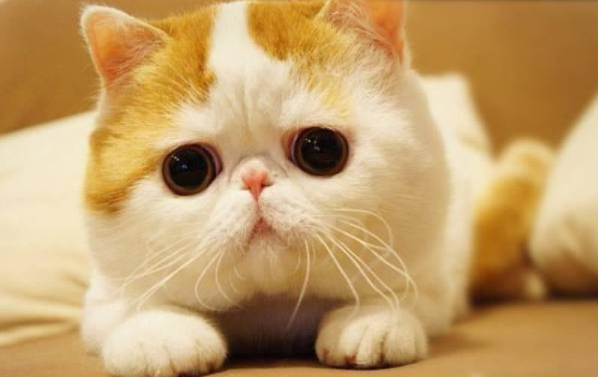
\includegraphics[width=0.5\textwidth]{Figuras/gatofofo.png}
	\fonte{Imagem ilustrativa (substitua pela fonte real da imagem).}
\end{figure}

Você também pode usar subfiguras para deixar o documento mais organizado. A Figura~\ref{fig_subfigname} ilustra um exemplo. Para citar uma subfigura específica, use \ref{subfig_cutecat} ou \ref{subfig_cutestdog}.

\begin{figure}[htb]
	\centering
	\caption{Animais de estimação fofos.}
	\label{fig_subfigname}
	\begin{subfigure}{0.3\textwidth}
		\centering
		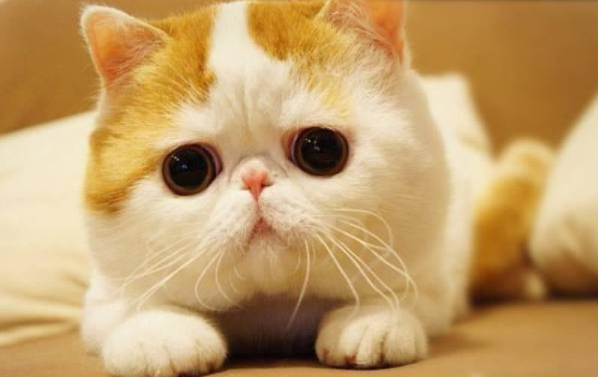
\includegraphics[width=\textwidth]{Figuras/gatofofo.png}
		\caption{Gato fofo.}
		\label{subfig_cutecat}
	\end{subfigure}\qquad
	\begin{subfigure}{0.3\textwidth}
		\centering
		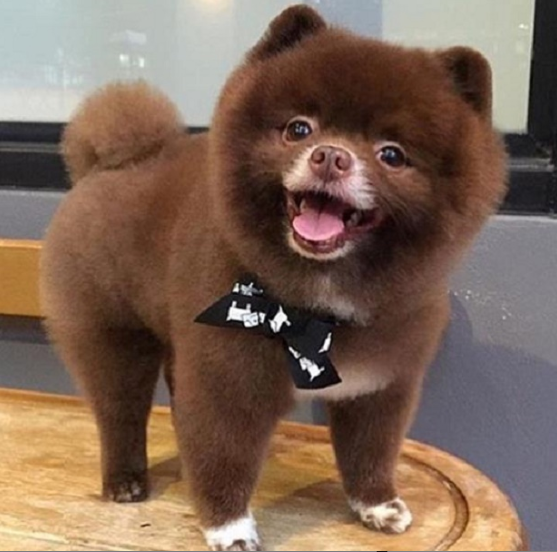
\includegraphics[width=\textwidth]{Figuras/cachorrofofo.png}
		\caption{Cachorro fofo.}
		\label{subfig_cutestdog}
	\end{subfigure}
	\fonte{Imagens ilustrativas (substitua pela fonte real das imagens).}
\end{figure}

%-----------------------------------
\section{Quadros: saídas, comandos e códigos}

Trechos de arquivos de configuração, saídas de comandos e códigos são conteúdo textual e devem ser apresentados como quadro, conforme o Quadro~\ref{qua_exemplocomando}.

\begin{quadro}[htb]
	\centering
	\caption{Listagem de arquivos gerados na compilação.}
	\label{qua_exemplocomando}
\begin{Verbatim}[fontsize=\small,frame=single]
$ ls main*
-rw-r--r--  1 autor users   3650 set 12 17:56 main.aux
-rw-r--r--  1 autor users   6366 set 12 17:43 main.bbl
-rw-r--r--  1 autor users    290 set 12 17:56 main.lof
-rw-r--r--  1 autor users  27937 set 12 17:56 main.log
-rw-r--r--  1 autor users    194 set 12 17:56 main.lot
-rw-r--r--  1 autor users    715 set 12 17:56 main.out
-rw-r--r--  1 autor users 159243 set 12 17:56 main.pdf
-rw-r--r--  1 autor users   4559 set 12 17:47 main.tex
-rw-r--r--  1 autor users    964 set 12 17:56 main.toc
\end{Verbatim}
%$ - esse comentário é para não confundir o realce de sintaxe do editor
	\fonte{Elaborado pelo autor.}
\end{quadro}

%-----------------------------------
\section{Tabelas}
\label{sec_tabelas}

A Tabela~\ref{tab_shorttable} apresenta o modelo de tabela que deve ser usado. Tabelas não têm bordas verticais nem fechamento lateral, e números devem manter a mesma quantidade de casas decimais, alinhados à direita; o texto deve ser alinhado à esquerda.

A ferramenta \texttt{Tables Generator}, disponível em \url{https://www.tablesgenerator.com/}, ajuda na construção de tabelas.

\begin{table}[htb]
	\centering
	\caption{Exemplo de tabela.}
	\label{tab_shorttable}
	\begin{tabular}{lrrr}
		\toprule
		Descrição    & \multicolumn{1}{c}{Valor 1} & \multicolumn{1}{c}{Valor 2} & \multicolumn{1}{c}{Valor 3} \\
		\midrule
		Aplicativo 1 & 1.352,70 &   1,22 &  1.358,00 \\
		Aplicativo 2 & 2.005,00 &  75,21 &  6.873,11 \\
		Aplicativo 3 & 8.648,00 &   5,45 &    852,00 \\
		Aplicativo 4 & 4.587,55 & 153,00 & 53.468,00 \\
		Aplicativo 5 &     0,00 &   0,00 &      0,00 \\
		\bottomrule
	\end{tabular}
	\fonte{Elaborado pelo autor.}
\end{table}

Para fazer referência a elementos que estão no apêndice, use: Tabela~\ref{tab_longtable} (Apêndice~\ref{apendiceA}).

Para fazer referência a elementos que estão no anexo, use: Anexo~\ref{anexoA}.

%-----------------------------------
\section{Algoritmos}
\label{sec_algoritmos}

O Algoritmo~\ref{alg:1} apresenta o pseudocódigo desenvolvido.

\begin{algorithm}[H]
	\SetAlgoLined
	\KwResult{Escreva aqui o resultado}
	inicialização\;
	\While{condição}{
		instruções\;
		\eIf{condição}{
			instrução1\;
			instrução2\;
		}{
			instrução3\;
		}
	}
	\caption{Como escrever algoritmos}
	\label{alg:1}
\end{algorithm}

\chapter{Metodologia}
\label{cap3_metodologia}

% Substitua este texto pela metodologia do seu trabalho.
Descreva o tipo de pesquisa (por exemplo, aplicada, exploratória, descritiva), a abordagem (qualitativa, quantitativa ou mista) e os procedimentos técnicos adotados (pesquisa bibliográfica, estudo de caso, experimento, desenvolvimento de software, entre outros).

Apresente as etapas executadas, os materiais, as ferramentas, as tecnologias e os dados utilizados, bem como os critérios e as métricas de avaliação, com detalhes suficientes para que outro pesquisador possa reproduzir o trabalho.

\chapter{Resultados e Discussão}
\label{cap4_resultados}

% ---------------------------------------------------------------
% ORIENTAÇÃO: se o seu trabalho tiver um capítulo intermediário
% (por exemplo, "Desenvolvimento do sistema" ou "O caso"), crie um
% novo arquivo em Capitulos/ e inclua-o no main.tex antes deste.
% Se os resultados forem extensos, a discussão pode virar um
% capítulo próprio.
% ---------------------------------------------------------------

Este capítulo apresenta os resultados obtidos e os discute à luz dos objetivos e da literatura.

\section{Apresentação dos resultados}
\label{sec_res_apresentacao}

Apresente os resultados de forma objetiva, organizados por objetivo específico ou por questão de pesquisa. Use figuras, quadros e tabelas sempre que facilitarem a compreensão, e cite cada um no texto antes de ele aparecer, comentando o que deve ser observado. Os exemplos do Capítulo~\ref{cap2_fundamentacao} mostram formas usuais de apresentação para cada tipo de trabalho, como a Tabela~\ref{tab_resultados_experimento} e a Figura~\ref{fig_likert}.

\section{Discussão}
\label{sec_res_discussao}

Interprete os resultados: o que eles significam, se respondem à questão de pesquisa, se confirmam ou contrariam os trabalhos relacionados (Seção~\ref{sec_trabalhos_relacionados}) e quais as suas implicações práticas. A discussão é o que diferencia uma monografia de um relatório técnico.

\section{Ameaças à validade}
\label{sec_res_ameacas}

Descreva os fatores que podem ter influenciado os resultados e o que foi feito para reduzi-los, por exemplo: tamanho e representatividade da amostra, viés do pesquisador, configuração do ambiente de testes e possibilidade de generalização dos resultados \cite{wohlin2012experimentation}.

\chapter{Conclusão}
\label{cap5_conclusao}

% Substitua este texto pela conclusão do seu trabalho.
Retome o problema de pesquisa e os objetivos apresentados no Capítulo~\ref{cap1_introducao}, indicando de que forma foram atendidos. Sintetize as principais contribuições do trabalho sem introduzir dados novos.

Por fim, apresente as limitações encontradas e sugestões de trabalhos futuros.


%-----------------------------------
% Finaliza a parte no bookmark do PDF
\phantompart

%-----------------------------------
% ELEMENTOS PÓS-TEXTUAIS (ordem da NBR 14724)
%-----------------------------------
\postextual

% Referências
\bibliography{referencias}

% Apêndices
% Apêndices: textos ou documentos elaborados pelo próprio autor
%-----------------------------------
\begin{apendicesenv}
\label{apendice}

%-----------------------------------
\chapter{Guia de uso do modelo LaTeX}
\label{apA_guia}

% Remova este apêndice da versão final do seu TCC.

Este apêndice resume como usar os principais recursos do modelo. A estrutura de arquivos e as instruções de compilação estão no arquivo \texttt{README.md} do projeto.

\section{Citações (ABNT NBR 10520:2023)}

A norma define as seguintes modalidades de citação:

\begin{alineas}
	\item citação direta: transcrição textual de parte da obra consultada;
	\item citação indireta: texto baseado na obra consultada;
	\item citação de citação: citação de um texto ao qual não se teve acesso ao original.
\end{alineas}

O comando \verb|\citeonline{chave}| gera a citação com o autor no corpo da frase, e \verb|\cite{chave}|, a citação entre parênteses:

\begin{enumerate}
	\item O aprendizado profundo é, segundo \citeonline{Lecun2015DeepLearning}, um subcampo do aprendizado de máquina que aprende representações em múltiplos níveis de abstração.
	\item A diversidade entre modelos pode ser obtida com conjuntos de treinamento ou hiperparâmetros diferentes \cite{Polikar2012EnsembleLearning}.
\end{enumerate}

Nas citações diretas, a página é obrigatória: \verb|\cite[p.~436]{chave}|. Citações diretas de até três linhas ficam entre aspas duplas, geradas com \verb|\enquote{...}|. Exemplo ilustrativo: segundo \citeonline[p.~436]{Lecun2015DeepLearning}, o aprendizado profundo \enquote{permite que modelos computacionais compostos de múltiplas camadas aprendam representações de dados}.

Citações diretas com mais de três linhas usam o ambiente \texttt{citacao}, com recuo de 4~cm, letra menor e sem aspas:

\begin{citacao}
For example, if the probability of an event is not known with precision, then it may be characterized linguistically as, say, quite likely, not very unlikely, highly unlikely, etc., where quite likely, not very unlikely and highly unlikely are interpreted as labels of fuzzy subsets of the unit interval \cite[p.~202]{zadeh1976fuzzy}.
\end{citacao}

A versão de 2023 da norma usa letras maiúsculas e minúsculas no nome do autor também entre parênteses; o pacote \texttt{abntex2cite} ainda gera caixa alta (padrão de 2002). Confirme com o orientador qual versão o curso adota.

As referências ficam no arquivo \texttt{referencias.bib}, e apenas as obras citadas aparecem na lista de referências. Páginas web devem ter os campos \texttt{url} e \texttt{urlaccessdate}, como a referência ao pacote abnTeX2 \cite{abntex2ctan}.

\section{Notas de rodapé e links}

Notas de rodapé são criadas com \verb|\footnote{...}|, sem espaço antes do comando e após a pontuação.\footnote{Exemplo de nota de rodapé.} Endereços são inseridos com \verb|\url{...}|, como \url{https://ctan.org/pkg/abntex2}, e links com texto, com \verb|\href{endereço}{texto}|, como a página do \href{https://ctan.org/pkg/abntex2}{abnTeX2}.

\section{Ilustrações e tabelas}

Toda ilustração (figura, quadro, gráfico) e toda tabela deve ter título acima, fonte abaixo (comando \verb|\fonte{...}|) e ser citada no texto antes de aparecer. Use rótulos com prefixos sugestivos (\texttt{fig\_}, \texttt{qua\_}, \texttt{tab\_}, \texttt{eq\_}) e referencie com til para evitar quebra de linha, como em \verb|Figura~\ref{fig_classes}|. Os exemplos deste modelo estão no Capítulo~\ref{cap2_fundamentacao}:

\begin{alineas}
	\item figuras desenhadas em TikZ: Figuras~\ref{fig_classes}, \ref{fig_likert} e \ref{fig_prisma};
	\item subfiguras: Figura~\ref{fig_processos};
	\item quadros, que apresentam informações textuais e têm bordas fechadas: Quadros~\ref{qua_classificacao} e \ref{qua_comparativo};
	\item tabelas, que apresentam dados numéricos e não têm bordas laterais: Tabelas~\ref{tab_requisitos} e \ref{tab_resultados_experimento};
	\item equações: Equações~\eqref{eq_media} e \eqref{eq_desvio};
	\item algoritmos: Algoritmo~\ref{alg_medicao};
	\item códigos-fonte, com o ambiente \texttt{lstlisting} dentro do ambiente \texttt{codigo}: Código~\ref{cod_agendamento};
	\item tabela longa, que continua em várias páginas: Tabela~\ref{tab_requisitos_completos}.
\end{alineas}

Imagens externas (PNG, JPG ou PDF) devem ser colocadas na pasta \texttt{Figuras/} e inseridas conforme o Quadro~\ref{qua_codigo_figura}. Não use imagens protegidas por direitos autorais sem autorização.

\begin{quadro}[htb]
	\centering
	\caption{Código para inserir uma figura a partir de arquivo.}
	\label{qua_codigo_figura}
\begin{Verbatim}[fontsize=\small,frame=single]
\begin{figure}[htb]
    \centering
    \caption{Título da figura.}
    \label{fig_exemplo}
    \includegraphics[width=0.6\textwidth]{Figuras/exemplo.png}
    \fonte{Elaborado pelo autor.}
\end{figure}
\end{Verbatim}
	\fonte{Elaborado pelo autor.}
\end{quadro}

\section{Versão para impressão}

Os links do PDF são coloridos para leitura em tela. Para gerar a versão impressa com links em preto, troque, no arquivo \texttt{main.tex}, a linha \verb|\impressaofalse| pela linha \verb|\impressaotrue|.

\section{Lista de verificação antes da entrega}

Antes de entregar o trabalho ao orientador ou à banca, confira os itens do Quadro~\ref{qua_checklist}.

\begin{quadro}[htb]
	\centering
	\caption{Lista de verificação antes da entrega.}
	\label{qua_checklist}
	\small
	\begin{tabularx}{\textwidth}{|c|X|}
		\hline
		\textbf{OK} & \textbf{Item} \\ \hline
		( \quad ) & Dados do trabalho preenchidos no \texttt{main.tex} (título, autor, orientador, ano). \\ \hline
		( \quad ) & Resumo com 150 a 500 palavras, em parágrafo único, seguido das palavras-chave separadas por ponto e vírgula; \textit{abstract} correspondente. \\ \hline
		( \quad ) & Todos os objetivos específicos retomados nas considerações finais. \\ \hline
		( \quad ) & Toda ilustração e tabela citada no texto antes de aparecer, com título acima e fonte abaixo. \\ \hline
		( \quad ) & Toda citação com entrada nas referências, e toda referência citada no texto; citações diretas com página. \\ \hline
		( \quad ) & Referências conferidas: autor, título, edição, local, editora, ano e, para páginas web, endereço e data de acesso. \\ \hline
		( \quad ) & Siglas e símbolos usados no texto presentes nas listas, e listas sem itens não usados. \\ \hline
		( \quad ) & Seções e apêndices de exemplo deste modelo removidos, incluindo as Seções~\ref{sec_como_usar} e \ref{sec_escolha_tipo} e este apêndice. \\ \hline
		( \quad ) & Listas vazias (de códigos, quadros, símbolos) removidas do \texttt{main.tex}. \\ \hline
		( \quad ) & Compilação sem erros e sem \enquote{??} no PDF (citações ou referências indefinidas). \\ \hline
		( \quad ) & Ficha catalográfica solicitada à biblioteca, para a versão final. \\ \hline
	\end{tabularx}
	\fonte{Elaborado pelo autor.}
\end{quadro}

%-----------------------------------
\chapter{Documento de requisitos (exemplo)}
\label{apB_requisitos}

Este apêndice exemplifica o documento de requisitos completo de um TCC de desenvolvimento de software (Seção~\ref{sec_tipo_desenvolvimento}) e o uso de tabela longa, que continua automaticamente nas páginas seguintes.

{\small
\begin{longtable}{@{}l p{9.5cm} l@{}}
	\caption{Requisitos do sistema de agendamento (exemplo).} \label{tab_requisitos_completos} \\
	\toprule
	ID & Descrição & Prioridade \\
	\midrule
	\endfirsthead
	\multicolumn{3}{c}{\tablename\ \thetable\ -- \textit{continuação}} \\
	\toprule
	ID & Descrição & Prioridade \\
	\midrule
	\endhead
	\midrule
	\multicolumn{3}{r}{\textit{Continua na próxima página}} \\
	\endfoot
	\bottomrule
	\multicolumn{3}{l}{\fontename: Elaborado pelo autor.} \\
	\endlastfoot
	\multicolumn{3}{l}{\textit{Requisitos funcionais}} \\
	RF01 & O sistema deve permitir o cadastro de clientes. & Alta \\
	RF02 & O sistema deve permitir agendar, remarcar e cancelar atendimentos. & Alta \\
	RF03 & O sistema deve enviar lembrete ao cliente um dia antes do atendimento. & Média \\
	RF04 & O sistema deve emitir relatório mensal de atendimentos. & Baixa \\
	RF05 & O sistema deve permitir o cadastro de serviços, com descrição e duração. & Alta \\
	RF06 & O sistema deve exibir a agenda diária e semanal de cada profissional. & Alta \\
	RF07 & O sistema deve impedir agendamentos em horários já ocupados. & Alta \\
	RF08 & O sistema deve permitir que o cliente consulte seus agendamentos. & Média \\
	RF09 & O sistema deve registrar o histórico de atendimentos de cada cliente. & Média \\
	RF10 & O sistema deve permitir a exportação de relatórios em PDF. & Baixa \\
	\midrule
	\multicolumn{3}{l}{\textit{Requisitos não funcionais}} \\
	RNF01 & O sistema deve funcionar nos navegadores Chrome, Firefox e Edge atuais. & Alta \\
	RNF02 & O sistema deve responder às consultas em até 2 segundos. & Média \\
	RNF03 & O sistema deve exigir autenticação com senha para acesso administrativo. & Alta \\
	RNF04 & O sistema deve tratar dados pessoais conforme a LGPD. & Alta \\
	RNF05 & A interface deve ser responsiva, adaptando-se a celulares. & Média \\
\end{longtable}
}

%-----------------------------------
\chapter{Questionário e TCLE (exemplo)}
\label{apC_questionario}

Este apêndice exemplifica os instrumentos usados em pesquisas com participantes, como \textit{surveys} (Seção~\ref{sec_tipo_survey}) e avaliações de sistemas com usuários. Adapte o texto às exigências do CEP, quando aplicável.

\section{Termo de Consentimento Livre e Esclarecido}

Você está sendo convidado(a) a participar da pesquisa \enquote{\imprimirtitulo}, desenvolvida por \imprimirautor, estudante do curso de Bacharelado em Sistemas de Informação do IFNMG -- Campus Salinas, sob orientação de \imprimirorientador.

\textbf{Objetivo}: descreva em linguagem simples o objetivo da pesquisa.

\textbf{Procedimento}: sua participação consiste em responder a um questionário com duração aproximada de 10 minutos.

\textbf{Riscos e benefícios}: descreva os riscos (por exemplo, desconforto ao responder alguma pergunta) e os benefícios esperados.

\textbf{Sigilo}: as respostas são anônimas e serão usadas apenas para fins acadêmicos, conforme a Lei Geral de Proteção de Dados Pessoais (LGPD).

\textbf{Participação voluntária}: você pode desistir a qualquer momento, sem qualquer prejuízo.

\textbf{Contato}: informe o e-mail do pesquisador responsável.

\vspace{0.5cm}
\noindent ( \quad ) Declaro que li e concordo em participar da pesquisa.

\section{Questionário}

\textbf{Parte 1 -- Perfil do respondente}

\begin{enumerate}
	\item Idade: ( \quad ) até 20 anos \quad ( \quad ) 21 a 30 anos \quad ( \quad ) 31 a 40 anos \quad ( \quad ) mais de 40 anos
	\item Com que frequência você usa o sistema? ( \quad ) diariamente \quad ( \quad ) semanalmente \quad ( \quad ) raramente
\end{enumerate}

\textbf{Parte 2 -- Avaliação} (1 = discordo totalmente; 5 = concordo totalmente)

\begin{table}[htb]
	\centering
	\caption{Afirmações do questionário (exemplo).}
	\label{tab_questionario}
	\begin{tabularx}{\textwidth}{Xccccc}
		\toprule
		Afirmação & 1 & 2 & 3 & 4 & 5 \\
		\midrule
		O sistema é fácil de usar. & ( ) & ( ) & ( ) & ( ) & ( ) \\
		O sistema é rápido. & ( ) & ( ) & ( ) & ( ) & ( ) \\
		O sistema atende às minhas necessidades. & ( ) & ( ) & ( ) & ( ) & ( ) \\
		\bottomrule
	\end{tabularx}
	\fonte{Elaborado pelo autor.}
\end{table}

\textbf{Parte 3 -- Questão aberta}

\begin{enumerate}
	\setcounter{enumi}{2}
	\item Que melhorias você sugere para o sistema?
\end{enumerate}

%-----------------------------------
\chapter{Roteiro de entrevista (exemplo)}
\label{apD_roteiro}

Este apêndice exemplifica um roteiro de entrevista semiestruturada, usado em estudos de caso (Seção~\ref{sec_tipo_estudo_caso}) e pesquisas qualitativas. Em entrevistas semiestruturadas, o roteiro orienta a conversa, mas o entrevistador pode acrescentar perguntas conforme as respostas.

\textbf{Abertura}: apresentar o objetivo da pesquisa, solicitar autorização para gravação e confirmar o consentimento do participante.

\textbf{Bloco 1 -- Perfil}

\begin{enumerate}
	\item Qual é a sua função na organização e há quanto tempo a exerce?
	\item Quais sistemas você utiliza no dia a dia?
\end{enumerate}

\textbf{Bloco 2 -- Processo atual}

\begin{enumerate}
	\setcounter{enumi}{2}
	\item Descreva, passo a passo, como o processo é realizado hoje.
	\item Quais são as principais dificuldades desse processo?
	\item Que informações você precisa e não consegue obter facilmente?
\end{enumerate}

\textbf{Bloco 3 -- Expectativas}

\begin{enumerate}
	\setcounter{enumi}{5}
	\item O que mudaria nesse processo, se pudesse?
	\item Como avaliaria uma solução informatizada para esse problema?
\end{enumerate}

\textbf{Encerramento}: agradecer a participação e perguntar se o participante deseja acrescentar algo.


\end{apendicesenv}


% Anexos
% Elemento opcional: texto ou documento NÃO elaborado pelo autor
%-----------------------------------
\begin{anexosenv}
\label{anexos}

%-----------------------------------
\chapter{Exemplo de anexo}
\label{anexoA}

Anexos reúnem documentos não elaborados pelo autor (por exemplo, normas, formulários ou manuais de terceiros) que servem de fundamentação, comprovação ou ilustração. Inclua-os, preferencialmente, como PDF:

\begin{verbatim}
\includepdf[pages=-]{Anexos/documento.pdf} % pacote pdfpages
\end{verbatim}

Toda figura inserida em anexo deve indicar a fonte e respeitar os direitos autorais da obra original.

\end{anexosenv}


\end{document}
